\chapter*{\LaTeX Tutorial}

The following is an introduction to some of the basic utilities of \LaTeX. While this tutorial may not answer all of your questions, the good news is that \LaTeX is widely used enough that the answer is probably out there somewhere! If you need additional help, you can consult:

\begin{itemize}
    \item Claire Warner (\url{cwarner@roclefeller.edu}) at the Rita \& Frits Markus Library
    \item Google! The internet is your friend, and it's almost guaranteed that someone has already asked your question before (and someone else has provided a solution). 
\end{itemize}

\section{Sections, Subsections, and Sub-Subsections} \label{sections}

You may want to organize your dissertation text by using a section hierarchy within your chapters. Sections, subsections, and sub-subsections will be automatically translated into the Table of Contents. Note that I have created a label for this section using the text. This means that if I want to reference Section \ref{sections} in other parts of the text, I can do so easily. This can also be done for subsections. If you swap the order of the sections in your text, all of the references will automatically have their numbers corrected.

\subsection{Subsection}

This is a subsection.

\subsubsection{Sub-Subsection}

This is a sub-subsection.

\section{Citing References}

You can cite references throughout your thesis. \LaTeX makes this easy through the use of a .bib file. The file called \url{references.bib} is where you will put all of the citations that you would like to reference in the main text of your dissertation. The references are in BibTeX format within the .bib file. There are several ways to automatically format references in this style:

\begin{enumerate}
    \item Use the Google Scholar Chrome extension. You can search for the desired article, click on ``Cite'' and select the BibTeX option. This will open a tab of plain text that can be copied and pasted into the .bib file.
    \item Use citation management software and export the desired citation(s) in BibTeX format. Note that while Zotero and Mendeley will do this easily, EndNote can cause more problems and will not automatically generate convenient citation keys. Once you have exported the citations, copy the text into the .bib file or upload the new file (if you do this, be sure to change the .bib file referenced in the main \url{thesis.tex} file).
    \item Link your citation manager directly to Overleaf. You can use this feature with either Mendeley or Zotero.
\end{enumerate}

Note that the references can be put into the .bib file in any order - they will automatically be formatted in the correct order when the References section is generated. To cite a reference in the text, simply type \url{\cite{key}}. Here, \url{key} is the citation key defined in the .bib entry for that citation. To cite multiple references at once, type \url{\cite{key1, key2}}. For example, \cite{anderson1995observation, schill2019water} and \cite{watson1953molecular} are the references used in this tutorial.

References will be enumerated in order of the first time they are cited. Citing them later in the text will maintain this numbering scheme and show the original citation number, like so: \cite{anderson1995observation}.

\section{Acronyms and Abbreviations}

You can add acronyms to the main text by writing something like the following: \acrlong{dna} (abbreviated \acrshort{dna}) is the molecule that carries genetic information for the development and functioning of an organism. This will populate the referenced acronym into the List of Acronyms in the front matter of your dissertation. Note that you must add the acronym to the \url{Abbreviations.tex} file \textbf{and} refer to it in the main text by its defined tag for it to appear in the List of Acronyms. The acronyms/abbreviations will appear listed in alphabetical order. Note that the List of Acronyms is an optional component of your dissertation. If you do not include it, be sure to define any acronyms or abbreviations where necessary in the text for clarity.

\section{Footnotes}

Here is an example of how to use footnotes. It is possible to write footnotes directly in the text itself \footnote{And type your footnote here.}. Or, mark the location of a footnote with footnote mark command\footnotemark \, and write the footnote on its own line. 

\footnotetext{Use the footnotetext command and write your footnote as previously.}

\section{Figures and Tables}

Figures and tables are important ways of visualizing data and conveying information. As always, be sure to cite figures and tables if they are not your own work, or if they have been featured in previous publications. \LaTeX provides environments for both figures and tables. Within each environment, you can specify the image file (or table contents and layout) as well as the title and caption. 

\subsection{Figures}

% This is a figure. Copy and paste this block of code for each figure. Change the width, image file path, title, and caption as needed. 
\begin{figure}
	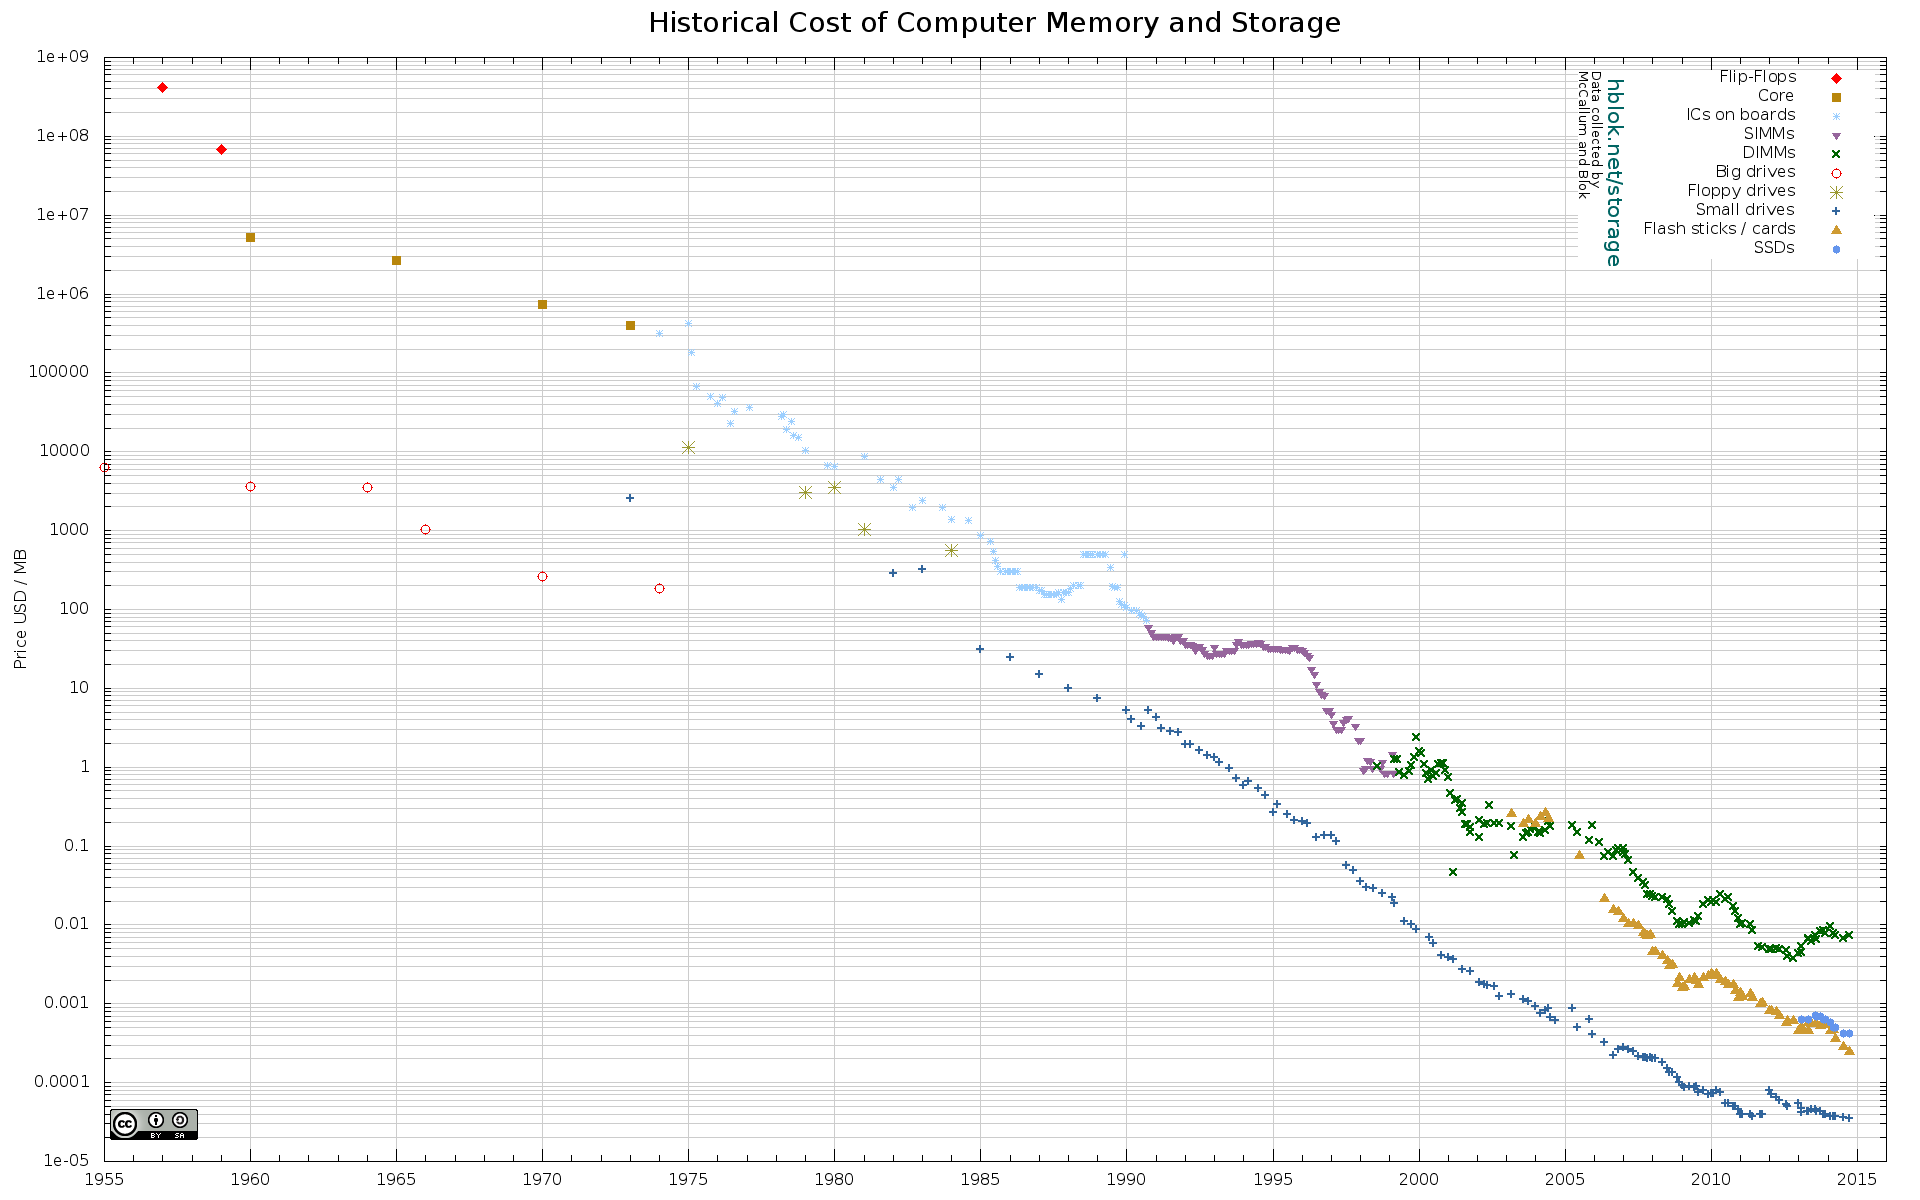
\includegraphics[width=\textwidth]{figures/exampleFigure.png} % Adjust width and file path as needed.
	\caption[Figure title for the Table of Contents]{ 
    Figure title for the main text. % By default, this should be identical to the figure title used in the Table of Contents.
    \textmd{Type a longer subtitle or caption here, optionally, which will appear unbolded in the main text.}
    }
	\label{fig:figurelabel} % Refer to this figure in the main text by typing \ref{figurelabel}. Be sure to give each figure a unique and sensible label.
\end{figure}

You should try to include figures close to where they are discussed in the text. You can refer to any figure, such as Figure \ref{fig:figurelabel}, in the text. Note that if you switch the order that figures are included in your \LaTeX code, the references in the text will automatically have their numbers updated, saving you a headache! You may wish to organize your image files in sub-folders. To do this, you can create sub-folders (for example, by chapter) within the ``figures'' folder and adjust the file path accordingly when using the \url{\includegraphics} command.


\subsection{Tables}

Tables are another important format for conveying both quantitative and qualitative information. First, begin the table environment using \url{\ begin{table} ... \ end{table}}. You can then define the captions for the Table of Contents and the main text in the same way as was done for figures. To begin to input the table, you must create a second environment called \url{tabular}. Immediately after the \url{\ begin{tabular}} command, you will define the shape of the table and the text alignment within the cells. In the example table shown, \url{ccc} specifies three columns with centered text and no vertical lines dividing them. To align the text left or right in a given column, simply type \url{l} or \url{r} instead of \url{c}. To place a vertical line between two columns, or on the edge of a column, use the ``|'' character in the appropriate location. For example, a table with a left- and a right-aligned column with borders and dividing lines would be \url{|l|r|}. 

You can then start filling in the contents of your table. The \url{&} character separates columns, and a double backslash indicates moving on to the line below. Typing \url{\ hline} will generate a horizontal line in your table. You can include equations or math characters in tables using \url{$ ... $}. You can further customize tables by merging columns or cells arbitrarily using the \url{\ multicolumn} command. If you are designing a complicated table, there are also many online tools that allow you to sketch out a table and generate the corresponding \LaTeX code!


% This is a table
% Adapt the number of figures and columns as needed.
\begin{table}
\caption[Table title for the Table of Contents]{ 
    Table title for the main text. % By default, this should be identical to the figure title used in the Table of Contents.
    \textmd{Type a longer subtitle or caption here, optionally, which appears unbolded in the main text.}
    }\begin{center}
\begin{tabular}{ccc}
Function & Form & $x$-derivative \\
\hline
Constant & $a$ & 0 \\
Linear & $ax + b$ & $a$  \\
Quadratic & $ax^2 + bx + c$ & $2ax + b$  \\
\label{tab:tablelabel}
\end{tabular}
\end{center}
\end{table}


\section{Labels}

Labels are an extremely useful feature of \LaTeX. They can be added to figures, tables, equations, or sections so that the labeled item can be referenced later in the text. To label an item, simply type \url{\ label{yourlabelhere}}. For large documents such as a dissertation, it can be helpful to develop a sensible naming scheme and to categorize your labels by type. For example, label your figures \url{\ label{fig:yourfiglabelhere}} and tables \url{\ label{tab:yourtablabelhere}}. This will help ensure you choose the right label when referencing items. To reference the figure number defined previously, simply type \url{\ ref{fig:yourfiglabelhere}}. As discussed in the next section, the method for referencing equations is slightly different and uses the \url{\ eqref{}} command. If you later decide to swap the order of two figures, \LaTeX will automatically update the numbers referenced throughout the text.

\section{Math and Equations}

One of the very best things about the \LaTeX language is its ability to format mathematical equations just the way you like them, with extensive options for mathematical symbols, Greek letters, super- and subscripts, and other special characters or mathematical operators. It also uses the same reference system as figures and tables, so that equations can be numbered and given a label that can be referenced throughout the text. Let's take a look at the Schrodinger Equation.

\begin{equation}
    i \hbar \frac{\partial \Psi }{\partial t} = \hat{H} \Psi
    \label{eq:schrodinger}
\end{equation}

From this one example, you can see a hint of the power provided by \LaTeX for equation editing. For more information on how to format equations, see this \href{https://en.wikibooks.org/wiki/LaTeX/Mathematics}{link}. You can reference equations like Equation \eqref{eq:schrodinger} like so. 

You may also like to use mathematical symbols in line with the main text. To do this, simply use the dollar sign to create a mini-math environment. Then you can easily discuss $\alpha$ cells, $\beta$-keratins, or $\gamma$-rays without skipping a beat.

\section{\LaTeX Quirks}

\subsection{Quotation Marks}

Since \LaTeX is a compiled typesetting language, it doesn't do some things that other software, such as Microsoft Word, might do automatically. One subtle but important example of this is quotation marks. While Microsoft Word will automatically format left- and right-facing quotation marks as needed, in \LaTeX you will need to distinguish between them with separate characters, as shown here for ``double quotes'' and `single quotes'. Note that the right-side double quote is created using two apostrophes ('') rather than the double quote character ("). 

\subsection{Special Characters}

You may quickly find that in writing your dissertation, you would like to use a character that is also used in the \LaTeX coding language. For example, the percent sign % will begin a comment
and the ampersand symbol lets you align text in equations. If you would like to use these, or other, special characters in your text, simply use a backslash, like so: \% \&. 